
%=====================================================================
% Document Style
%=====================================================================
% APS format: There is no prescribed format by IIT Bo\emph{}mbay
\documentclass{raitdisser}
% To include optional packages, use the \usepackage command.
% For e.g.:
\usepackage{graphicx}
%=======================================================================
% End of Preamble, start of document
%\begin{document}

% Choose your bibliography style
% plain is the basic style, others include ieeetr, siam, asm, etc
\bibliographystyle{plain}




%\include{defs}                   % Common definitions used throughout the thesis
%============================================================================
% prelude.tex
%   - titlepage
%   - table of contents, list of tables and list of figures
%   - abstract
%============================================================================
\clearpage%
\pagenumbering{roman}  % This makes the page numbers Roman (i, ii, etc)
%--------------------------------------------------------------------%
% TITLE PAGE
%   - define \title{} \author{} \date{}

\title{Analysis using Belief Propagation Techniques}
\author{Chitra Suresh}

\date{January 2015}

\department{Department of Electronics Engineering}

%    - Set the guide's name
\setguide{Prof.Dr.Kushal.R.Tuckley}
%    - Set the coguide's name (if you have one)
%%\setcoguide{Prof Amitabha Sanyal}

%   - once the above are defined, use \maketitle to generate the titlepage
\maketitle

%--------------------------------------------------------------------
\cleardoublepage \nonumber
%\begin{center}
%
\includegraphics{raitlogo.eps}\\
%Ramrao Adik Education Society's\\
%\large {\textbf{Ramrao Adik Institute of Technology}}\\
%\small(Affiliated to the University of Mumbai)\\
%Dr. D. Y. Patil Vidyanagar,Sector 7, Nerul, Navi Mumbai 400
%706.\\\vspace{0.3in} \Large CERTIFICATE
%\end{center}
%\vspace{0.1in}
%\begin{center}
%\large This to certify that Dissertation Seminar-I entitled\\
%\textbf{\lq\lq On Scheduling in WiMAX\rq\rq} \\submitted by
%\begin{center}
% w (09)\\
%\end{center}
%is approved for the degree of \\ \textbf {Master of Engineering}\\ in\\ \textbf {Electronics Engineering}.\\
%
% %\vspace{0.5in}
%%-----------------------------------------------------------------
%%\begin{tabular}{ccc}
%%      \rule{6cm}{1sp}                &\rule{10mm}{0pt}& \rule{6cm}{1sp}
%%      \\
%%       Guide             &&Head of Department \\\\\
%%      \rule{6cm}{1sp}                && \rule{6cm}{1sp} \\
%%      Examiner 1                 && Examiner 2 \\\\\\
%%      Principal: \rule{4cm}{1sp} && \\ && \\
%%       &&
%%    \end{tabular}
%\vspace{1in}
%\begin{tabular}{ccc}
%      \rule{5cm}{1sp}                &\rule{10mm}{0pt}& \rule{5cm}{1sp}
%      \\\vspace{0.5in}
%      Examiner 1                 && Examiner 2 \\
%      \rule{5cm}{1sp}                && \rule{5cm}{1sp} \\ \vspace{0.5in}
%       Guide             && Project Coordinator \\
%      \rule{5cm}{1sp}                && \rule{5cm}{1sp} \\
%      Head of Department                && Principal \\\\
%        %&\rule{5cm}{1sp}& \\
%%       &Principal&
%    \end{tabular}
%\end{center}
%-----------------------------------------------------------------
\cleardoublepage
%--------------------------------------------------------------------%


% ABSTRACT
\begin{abstract}
%\input {abstract}
Belief Propagation Techniques uses the degree of a person's belief that an event will occur,rather than the actual probability  of the event will occur.
Belief Propagation Technique is used to perform inference on graphical  model  such as factor graphs which calculates marginal distribution for each unobserved node
conditional on observed node.
Belief Propagation Techniques  are used for performing inference on graphical models such as Bayesian Network and Markov Random Field
\\Bayesian network uses the directed graphs where the directions of the arrows permits distinguish genuine dependencies for spurious dependencies induced by hypothetical observations
\\In Markov Random  Fields,the network topology was presumed to be given and problem was to characterize the probabilistic  behavior  of a system complying with dependencies prescribed by network.
\\Belief Propagation Techniques are used in  wide variety of algorithms which are used in Artificial intelligence,Signal processing and Digital communication.
\\Markov  Random Fields and  Bayesian Networks  methods are used  to optimize Belief Propagation  algorithm.
\\\ \textbf{ Keywords}:Belief Propagation Technique,Bayesian Network and Markov Random Field
\end{abstract}

%--------------------------------------------------------------------%
% CONTENTS, TABLES, FIGURES
%\tableofcontents
\listoffigures\

%--------------------------------------------------------------------%
%  Single counter for theorems and theorem-like environments:
\newtheorem{theorem}{Theorem}[chapter]
\newtheorem{assertion}[theorem]{Assertion}
\newtheorem{claim}[theorem]{Claim}
\newtheorem{conjecture}[theorem]{Conjecture}
\newtheorem{corollary}[theorem]{Corollary}
\newtheorem{definition}[theorem]{Definition}
\newtheorem{example}[theorem]{Example}
\newtheorem{figger}[theorem]{Figure}
\newtheorem{lemma}[theorem]{Lemma}
\newtheorem{prop}[theorem]{Proposition}
\newtheorem{remark}[theorem]{Remark}

%--------------------------------------------------------------------%
% Make the page numbers Arabic (1, 2, etc)
\cleardoublepage%
\pagenumbering{arabic}

              % Title page, abstract, table of contents, etc
\chapter{\textbf{Introduction}}
This report introduces Belief Propagation Techniques and presents some of the  applications.
\\ Belief Propagation Techniques approach uses the degree of a person's belief that an event will occur,rather than the actual probability  of the event will occur.
Belief probabilities are  properties of person's belief not the event.
\\ A Probabilistic model is a dependency model in which relationship between  each of the variable is captured.Dependency models  are represent by graphical methods.
\\ Belief Propagation Technique is used to perform inference on graphical  model  such as factor graphs which calculates marginal distribution for each unobserved node
conditional on observed node.
The graphical representation used for belief propagation Techniques are two types ,they are Markov  Random Fields and  Bayesian Networks.\cite{Hans Andrea Loeliger}
\\Belief Propagation Techniques  are used for performing inference on graphical models such as Bayesian Network and Markov Random Field\cite{Judea Pearl}
\\Bayesian network uses the directed graphs where the directions of the arrows permits distinguish genuine dependencies for spurious dependencies induced by hypothetical observations
\\In Markov Random  Fields,the network topology was presumed to be given and problem was to characterize the probabilistic  behavior  of a system complying with dependencies prescribed by network.
\\Belief Propagation Techniques are used in  Artificial Intelligence,Signal Processing and  Digital Communication.
\\Some of the applications where Markov  Random Fields and  Bayesian Networks  methods are used  either as  optimization tool or for implementation  are discussed in chapter 3

\begin{itemize}
 \item \textbf{Efficient Belief Propagation for Early Vision.}The method used in this application is Markov Random  Fields on the Belief Propagation to solve problems for low level vision.                                                                 \cite{Pedro}
  \item \textbf{Markov Network-based Unified Classifier for Face Identification} Markov Random  Fields is used  for face recognition for one to many identification task                        \cite{Wonjun}
  \item \textbf{Efficient Loopy Belief Propagation using the Four Color Theorem} Four Color Theorem is based on Max-Product Belief Propagation Technique can be used in solving Markov Random  Fields problems where energy is minimized.                     \cite{Radu}
  \item \textbf{Image Completion Using Efficient Belief Propagation Via Priority Scheduling and Dynamic Pruning}           \cite{Nikos}
\end{itemize}
\begin{itemize}
   \item  Belief propagation Algorithm is used in \textbf{Low Memory Cost Block-Based Belief Propagation For Stereo Correspondence}\cite{yuchang}
   \item Bayesian network method of graphical representation for \textbf{ Task Parallel Implementation of Belief Propagation
In Factor Graphs}\cite{Nam Ma}
   \item A graphical model such as the Markov random field (MRF) of Belief Propagation Technique is used in \textbf{Hardware-Efficient Belief Propagation}\cite{Chia-KaiLiang}
 \item A method of Particle Belief Propagation (PBP) is used in \textbf{PatchMatch Belief Propagation for
Correspondence Field Estimation.}\cite{F.BESSE}
 \item Continuous time  Bayesian network method is used in \textbf{Learning continuous time Bayesian network classifiers}\cite{Daniele}
\end{itemize}
The organization of report is as follows Introduction in \textbf{Chapter-1},Mathematics related to Belief Propagation Techniques is in \textbf{Chapter-2},Different applications related to Belief Propagation Techniques are in \textbf{Chapter-3},conclusion in \textbf{Chapter-4.}



            % Chapter 1: Introduction
\chapter{\textbf{Mathematics related to Belief Propagation Technique}}

\section{Probabilistic Formulation:}

Bayesian Methods provide a formalism for reasoning about partial beliefs under condition of uncertainty..
In the Bayesian formalism,beliefs measures obey the three basic axioms of probability theory.


\begin{equation*}
   0 \leq P(A) \leq 1
\end{equation*}

\begin{equation*}
    P(Sure Propositions)=1
\end{equation*}

\begin{equation*}
  P (A    or  B) = P(A)+ P(B)
\end{equation*}
 if A and B are mutually exclusive
\\The basic expressions in the Bayesian formalism are statement about conditional probabilities be that
the probability of any event A computed by conditioning it on any set of exhaustive and mutually exclusive events $B_i,i=1,2,......n$



\begin{equation*}
     P(A)= \sum \{P(A\setminus B_i)\times P(B_i)\}
\end{equation*}


This decomposition provides the basics for the hypothetical or assumption based reasoning in the bayesian formalism.It states that the belief in any event A is weighted sum over the beliefs in all the distinct  ways that event A might be realized.
\\ Another useful generalization of the product rule is so called \textbf{Chain Rule Formula}.
\begin{equation*}
P(A,B)=P(A|B)P(B)
\end{equation*}

It states that if  a set of n events $(E{_1},E{_2},......E{_n})$


then,the probability of joint event $(E_1,E{_2},......E{_n})$ can be write
ten as a product of n conditional probabilities.


\begin{equation*}
    P(E{_1},E{_2},......E{_n})=P(E_{n}|E_{n-1},......E{_2},E{_1})......P(E{_2}|E{_1})P(E{_1})
\end{equation*}
This product can be derived by repeated application of equation 2.5. in any convenient order.
\section{Probability Model}

A probability model is an encoding of the probabilistic information in some domain of interest,such that each well formed sentence,statement or proposition can be calculated in accordance with axioms of probability theory.
\\These sentences are represented by interrelating random or stochastic variables with in model.
\\The  probability model (M) is defined by the joint probability of all its variables or universe

%$\triangleq$

Each variable in a probabilistic model may take any one of a set of mutually exclusive or collectively
exhaustive states.
The random variable may be discrete or continuous.The discrete random variable has finite of possible states,the probability distribution of Discrete random variable is probability mass function whereas continuous random variable takes their state from an infinite set of possible values.The probability distribution of continuous random variable is probability density function.
\section{Probability Language}

Probability language is well suited to reasoning under uncertainty.It provide a suitable frame work for processing the uncertainty relationship between variables of a probabilistic model.
probability language provide consistency of inferred results and knowledge base through their axiomatic basis and provide a convenient mechanism for presenting uncertain results.
The basic four primitives of probability language are\begin{enumerate}
                                                      \item Likelihood
                                                      \item Conditioning
                                                      \item Relevance
                                                     \item Causation
                                                     \end{enumerate}

\begin{itemize}
  \item A likelihood of event  is measure of  how likely or probable it is that the event will occur ie.chance of occurrence.
  \item A conditioning :An event is conditional  second event ,if its  is changed by the knowledge of second event states.
  \item Relevance: events A and B are said to be relevant to each other in the context of event C ,if adding the knowledge of C to the knowledge of B,changes the likelihood of A.
  Example: Two events are relevance,when common sequences is observed.ie A and B are relevant if both are causes of C.
\item Causation conveys a pattern of dependence between events.
\end{itemize}

\section{Graphical Representation}
A probabilistic model is dependency model in which the relationship between each of the variable is captured.
A graph is denoted by G(V,E) is set of nodes or vertices V connected by the set of arcs or edge E.
Graphs may be used to represent dependency model
\\For example :Dependency Model M comprising the variables U represented by graph.
\\The set of arc E represents conditional dependencies between these variables.
\\ie.Joint probability function of M is encoded in E

%G $\triangleq$
%\triangleq {G{M}(U,E)}$
Nodes of the graph corresponds to variables in dependency model
U$\rightarrow$ variables
\paragraph\   Graphical representation for probabilistic model are two types one is undirected graph and directed graph.
Undirected graph had no explicit direction,an arc of influence between connected nodes
Examples of undirected graph is Markov Random Fields.
In directed graph arcs are either unidirectional or bidirectional directed arc provide the mechanism for representing causation
Example for Directed graph is Bayesian network
\paragraph{Markov Random Fields and Bayesian network are two types of graphical representation for probabilistic models}

\section{Bayesian Belief Network}
The Bayesian Belief Network(BBN)determines the state probabilities of each node or variable from predetermined conditional and prior probabilities.
The Direct Acyclic Graph(DAG) G(U,E)of the probability model M represents probability distribution P(U) ,where U represents set of all variables in M
\begin{equation}\label{}
   X{_1},X{_2},........X{_n}
\end{equation}
Variables in probability distribution P(U)
Direct Acyclic Graph(DAG) in which minimal set of variables are designed as parent of each variable
\X{i} such that
\begin{equation}\label{}
   P(X{_i}/W);   W\in{X{_1},X{_2}.....X{_{i-1}}}
\end{equation}

The above equation is BBN of that probability distribution
For DAG to be Bayesian network of M,it is necessary and sufficient that each variable be conditional independent of all of its non descendents given in parents also satisfies this condition.
\\\
In practice usually understands the constrains in the domain of interest.However easily identify the variables that directly influence other variables ie.eaiser to understand the local interaction of variables than the domain as a whole.
\\
The basic concept in the Bayesian treatment of uncertainties in causal network is conditional probability ie.
Given the event B,the probability of event A is x

\begin{equation}
    P(a / b) = x
\end{equation}
Conditional probability
\begin{equation}
    P(a/b)P(b)=P(a,b)
\end{equation}
In real world all events are conditioned by some context C=c
\begin{equation}
    P(a/b,c)P(b/c)=P(a,b/c)
\end{equation}
The Baye's rule also conditioned on
\begin{equation}
 P(b/a,c)={P(a/b,c)P(b/c)} / {P(a/c)}
\end{equation}
\begin{itemize}
  \item P(b/a,c) is posterior probability of b
  \item P(a/b,c) liklihood probability
  \item P(a/c) Normalized factor
  \item P(b/c) Priori probability of b
\end{itemize}
Normalised factor is not directly availableis replaced by
\begin{equation}\label{}
    \int_{b} P(a/b,c)p(b/c)db
\end{equation}
\begin{equation}
    \sum_{b}P(a/b,c)p(b/c)
\end{equation}

For continuous and discrete distributions


\section{Markov Field Belief Technique }
\ Markov  Random Field of Belief propagation Technique is used to convey information for useful decisions and for  inference problems.
\ Markov  Field of Belief propagation Technique can be expressed in terms of conditional independence of its non neighbors,once values of neighbors  are known.
\\ If assigning of weights to the links of the graph must be handled with caution.If the weights are to be used translating evidential data in to meaning full probabilistic inferences such probabilistic model is both consistent and complete.Consistency guarantees that,it don't over load the graph with too many parameters.


The theory of Markov fields provides a safe method for constructing a complete and consistent quantitative model while preserving the dependency structure for an arbitrary graph (G).\\


The method consists of four steps
\begin{enumerate}
  \item Identify the associates of G ,namely, the maximal subgraphs whose nodes are all adjacent to each other

% P(A)= \sum \{P(A\setminus $B_i$)\times P($B_i$)\}

   %\item For each associate $C{_i}$,assign a nonnegative compatibility function $g{_i}$$(c{_i}$ ,which measures the relative degree of compatibility associated with each value assignment c{$_i$}to the variable included in$ C{_i}$
  %\item Form the product \\prod{$_i$}g{$_i$}(c{$_i$}) of the compatibility functions over all associates.
 % \item Normalize the product of all possible value combinations of the variables of the system
\begin{equation}\label{}
    P( x{_i},....,x{_n}) =K\prod_{i}g{_i}(c{_i})
\end{equation}

where
 \begin{equation}\label{}
    K= 1\div[\sum_{x{_1},...x{_n}}\prod_{i}g{_i}(c{_i})]
 \end{equation}

\end{enumerate}












                   % Other chapters as required
\chapter{\textbf{Applications of Belief Propagation Techniques}}
Belief Propagation Technique is used for performing inference on graphical models such as Bayesian Network and Markov Random Fields.\\Belief Propagation Technique calculates marginal distribution for each unobserved node, conditioning on any unobserved node.\\Some of the applications where Belief Propagation Techniques are used explained below.

\section{Efficient Belief Propagation for Early Vision}

Markov random field models provide a robust and unified framework for early vision problems such as stereo and image restoration. Inference algorithms based on graph cuts and belief propagation have been found to yield accurate results, but despite recent advances are often too slow for practical use.\\ In this paper some of the techniques  are used that substantially improve the running time of the loopy belief propagation .
\begin{enumerate}
  \item One of the techniques reduces the complexity of the inference algorithm to be linear rather than quadratic in the number of possible labels for each pixel, which is important for problems such as image restoration that have a large label set.
  \item second  technique speeds up and reduces the memory requirements of belief propagation on grid graphs.
  \item  A third technique is a multi-grid method that makes it possible to obtain good results with a small fixed number of message passing iterations, independent of the size of the input images.
\end{enumerate}


Taken together these techniques speed up the standard algorithm by several orders of magnitude. In practice results  obtained   are as accurate as those of other global methods (e.g., using the Middlebury stereo benchmark) while being nearly as fast as purely local methods.
\\The three techniques are used for speeding up the belief propagation by using Markov random fields for solving low level vision problems.
\\\\\ \\ The time necessary to compute a single message update from O (k 2 ) to O (k), where k is the number of possible labels for each pixel for the max-product formulation ie.linear rather than quadratic is possible.
\\By using max-product formulation and by grid graphs , The fast message updates to arbitrary discontinuity cost functions based on difference between labels and labels are embedded in some space but do not lie on a regularly spaced grid can be enhanced .



\section{Markov Network-based Unified Classifier for Face Identification }
In this research paper ,a novel unifying framework using a Markov network to learn the relationship between multiple classifiers in face recognition is explored. \\A  several complementary classifiers and assign observation nodes to the features of a query image and hidden nodes to the features of gallery images. each hidden node is connected to its corresponding observation node and to the hidden nodes of other neighboring classifiers.\\ For each observation-hidden node pair, to  collect a set of gallery candidates that are most similar to the observation instance, and the relationship between the hidden nodes is captured in terms of the similarity matrix between the collected gallery images. Posterior probabilities in the hidden nodes are computed by the belief-propagation algorithm.\\ The novelty of the proposed framework is the method that takes into account the classifier dependency using the results of each neighboring classifier. The  two different evaluation protocols, known and unknown image variation tests, using three different databases, which shows that the proposed framework always leads to good accuracy in face recognition.\\

When  a face image is used as as a query,  can retrieve several desired face images from a large image database,then  calculate many similarities of the query image and the
gallery images in the database, and the retrieved gallery images are ranked by similar orders. \\It is a one-to-many identification problem  and has many applications such
as searching similar face images in a database and face tagging in images and videos.\
\\Recent successful face recognition methods have attempted to merge several classifiers using multiple feature sets of different characteristics, as in component-based methods, which extract features from separate spatial regions , and heterogeneous feature-based methods which merge different domain features. \ These methods used the classifiers not only based on the different feature sets but also trained independently, and the similarity scores are merged with the predefined parameters. The parameter comes from the training database and it is not the best choice when the input image has different conditions. Note that these methods lead to good accuracy in face verification, but there is no specific framework for the one-to-many identification problem.
\begin{figure}
  % Requires \usepackage{graphicx}
  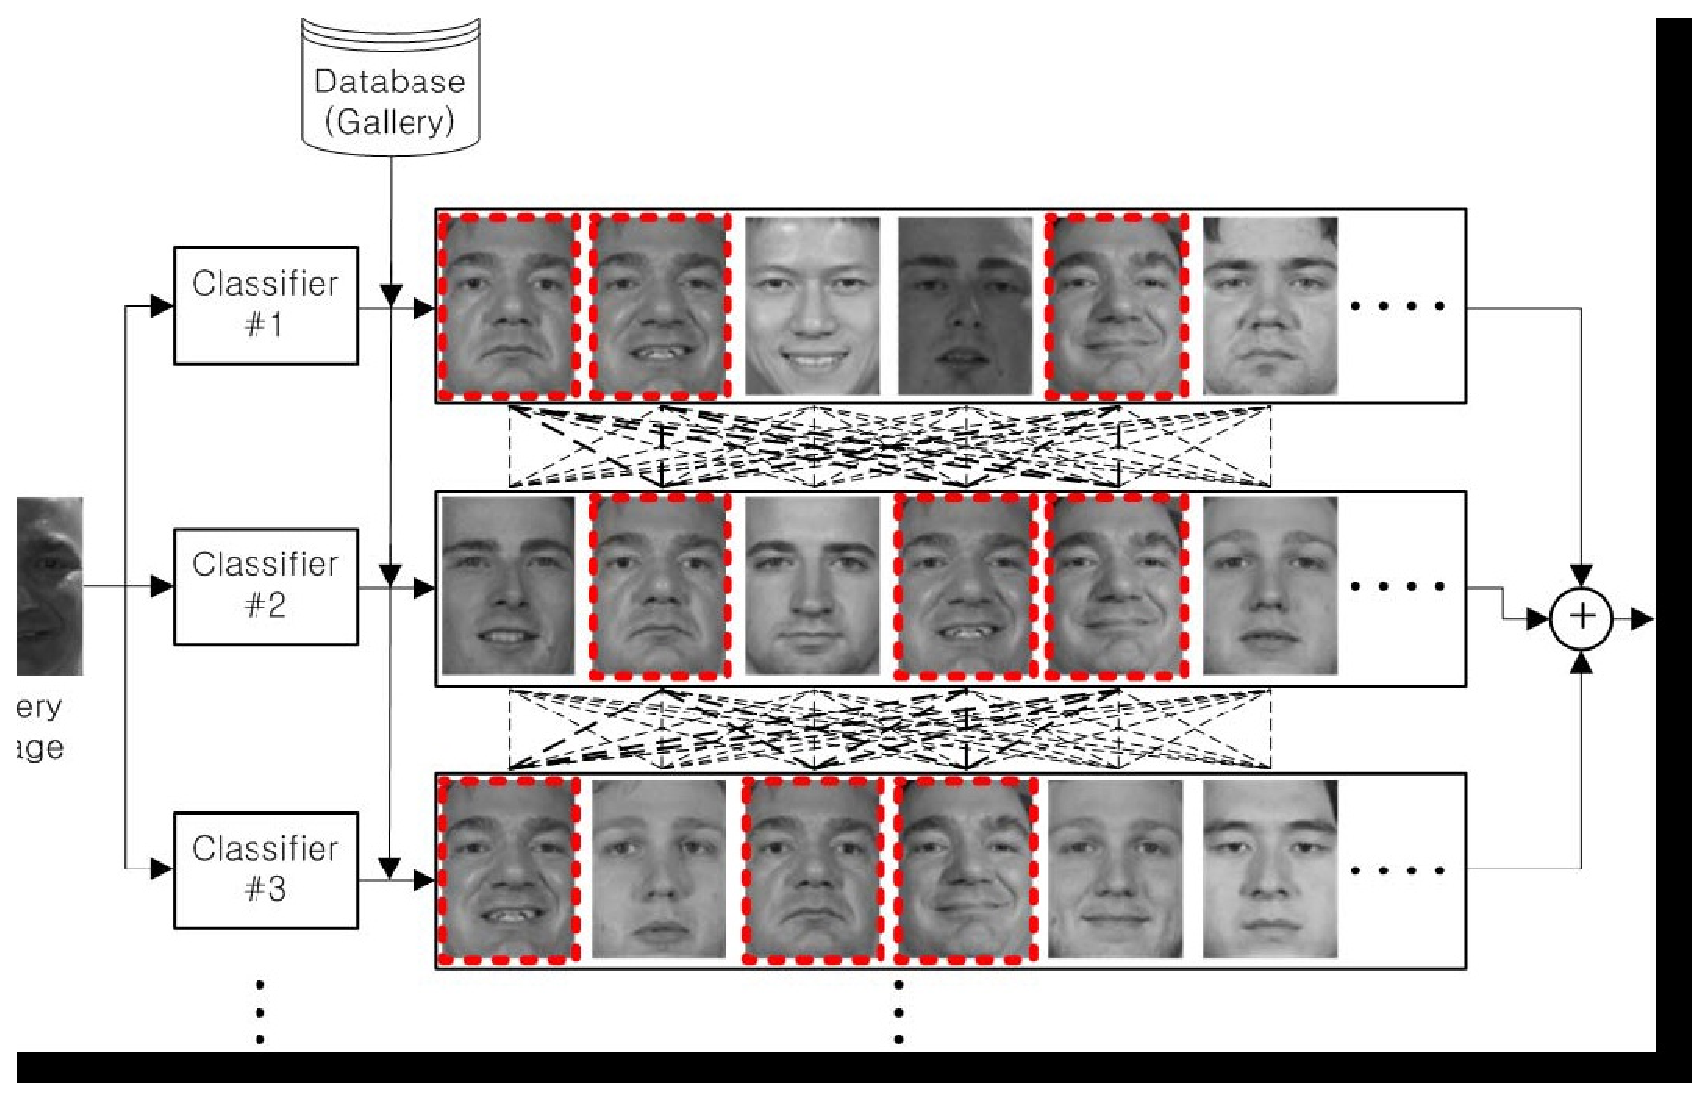
\includegraphics[width=4in]{face.eps}\\
  \caption{One-to-Many identification }\label{}
\end{figure}
\begin{figure}
  % Requires \usepackage{graphicx}
  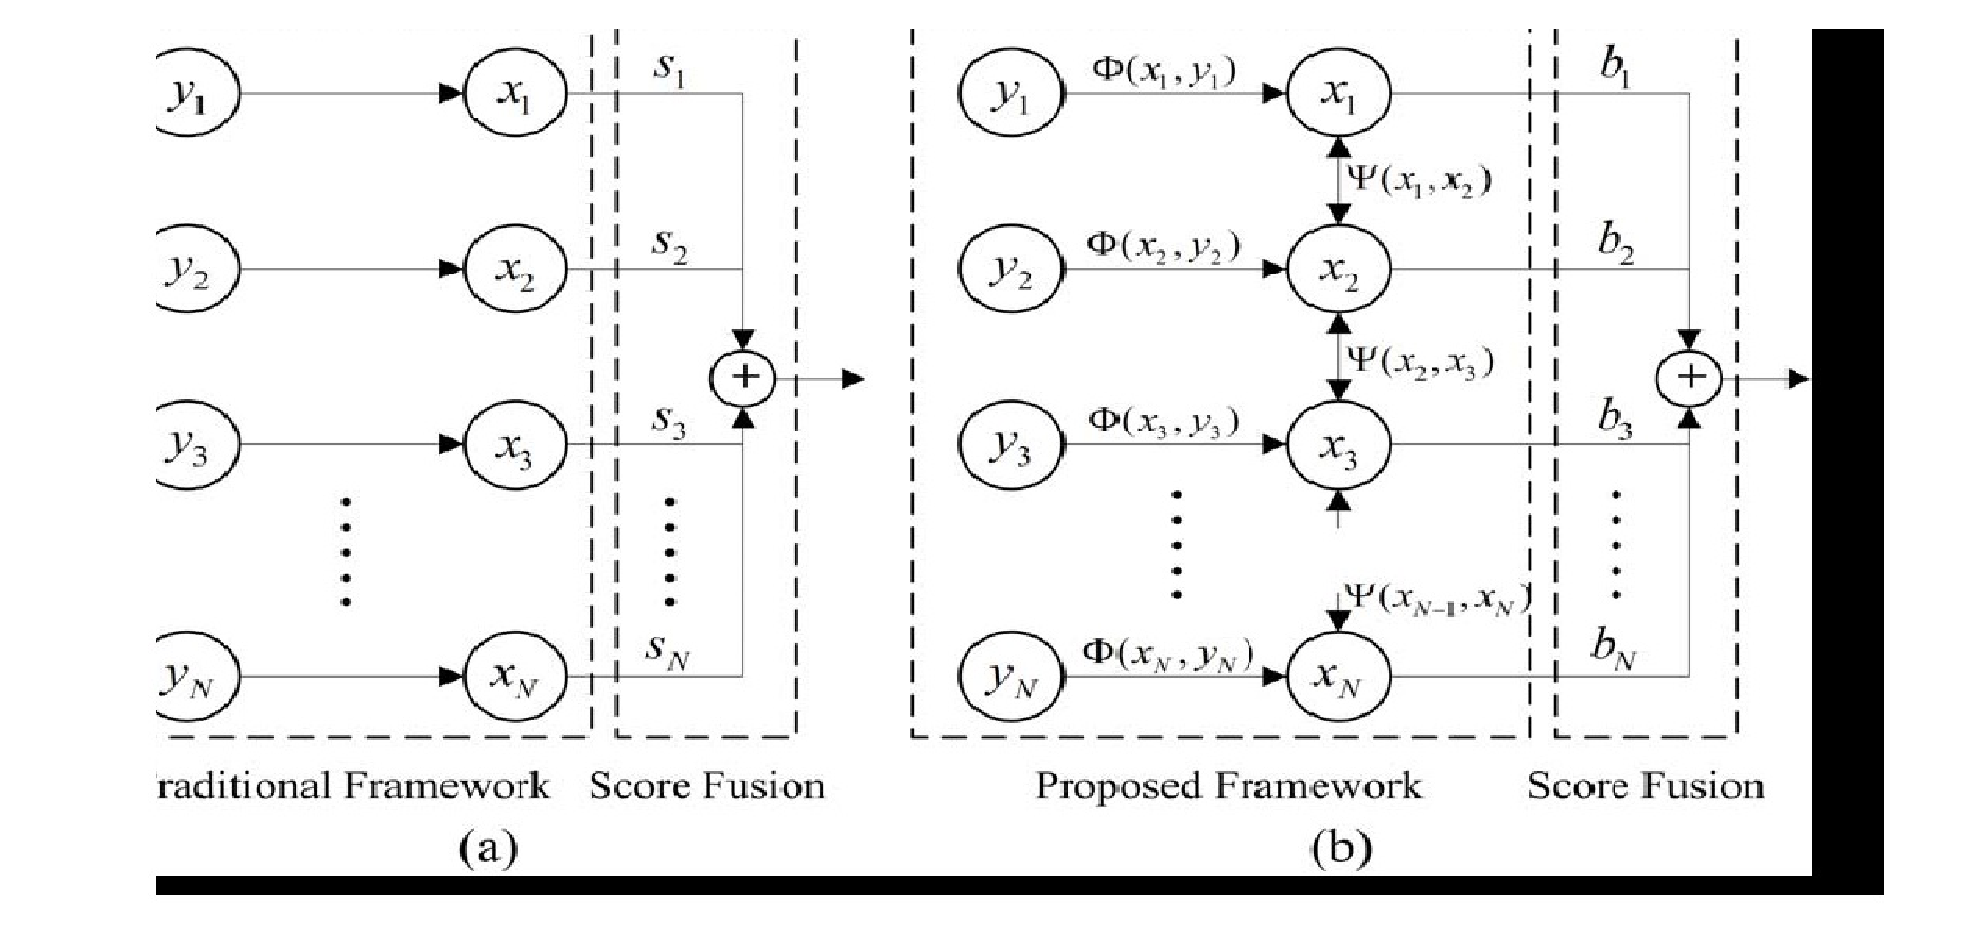
\includegraphics[width=4in]{classifier.eps}\\
  \caption{Traditional and proposed Frame Work}\label{}
\end{figure}

 \begin{itemize}
   \item In this paper, a novel recognition framework for the one-to-many identification issue is designed, and the simple concept is illustrated in Figure 3.1.
   \item First, assume that multiple classifiers have complementary characteristics, unify the multiple classifiers based not on the predefined weight values but on a Markov network, as summarized in Figure 3.2
 \end{itemize}

  For this purpose, assign one node of a Markov network to each classifier.The steps to find marginal probability by using Markov Fields for classifiers are as follows
  \begin{enumerate}
    \item Nodes are connected by lines, which represents the statistical dependencies
    \item For an observation node, we extract a feature from a query image using the corresponding classifier.
    \item At its paired hidden node,  the first retrieve n similar gallery samples from the database, and their orders are made by the similarity scores for the query face image.
  \item The multiple classifiers have their own lists of retrieved gallery images, which are not identical in general, thereby complementing the neighbor classifiers. Because the hidden nodes are connected by the network lines,
  \item The relationship of the connected nodes is learned by the similarity scores between the neighbor classifiers, and the scores are calculated by concatenating the two gallery features of the neighbor classifiers.
  \item The posterior probability at each hidden node is easily computed by the belief-propagation algorithm. Finally, marginal probability for a score value at each classifier is calculated
  \end{enumerate}
 And also analyze the generalizability of the method using different multiple classifiers such as the Random Sampled Gabor (RSG) method, which consists of the simple and weak classifiers, and the Extended Curvature Gabor (ECG) method which consists of more complex and stronger classifiers.
\\The results obtained are for face recognition particularly for the one-to-many identification task, based on multiple classifiers gallery connected by a Markov network.The Markov network probabilistically models the relationships between a query and images and between neighboring gallery images.
The observation-hidden node pair retrieve the  similar gallery images from the database image.
\\The similarities between the retrieved gallery images gives the statistical dependency between the hidden nodes. Hence results obtained can be viewed as clustering-based face recognition.



\section{Efficient Loopy Belief Propagation using the Four Color Theorem}
Recent work on early vision such as image segmentation, image  denoising, stereo matching, and optical flow uses Markov Random Fields.\\ Although this formulation yields an NP-hard energy minimization problem, good heuristics have been developed based on graph cuts and belief propagation.\\ Nevertheless both approaches still require tens of seconds to solve stereo problems on recent PCs. Such running times are impractical for optical flow and many image segmentation and
denoising problems and review on  recent techniques for speeding them up.

Moreover in this research paper it shows that  how to reduce the computational complexity of belief propagation by applying the Four Color Theorem (FCT) to limit the maximum number of labels in the underlying image segmentation to at most four. This provides substantial speed improvements for large inputs, and this for a variety of vision problems, while maintaining competitive result quality.
\\\\\\ In this research paper two methods are developed based on graph cuts  and belief propagation .

 \begin{itemize}
   \item In the case of Belief Propagation (BP), a key reason for its slow performance is that the algorithm complexity is proportional to both the number
of pixels in the image, and the number of labels in the underlying image segmentation
which is typically high. If  limit the number of labels, its speed performance should improve greatly.
   \item
By modifying the propagation algorithms like can using a low number of placeholder
labels, that can reuse for non-adjacent segments. These placeholder labels
can then be replaced by the full set of actual labels.
   \item Since image segments
form a planar graph, they therefore require at most four placeholder labels by
virtue of the Four Color Theorem (FCT)  to still have different colors for
all adjacent segments.
 \item A joint optimization process provides a fast segmentation
through the placeholder labels and a fine grained labeling through the
actual labels.
 \item  The computational time is basically dependent on the number
of placeholder rather than actual labels.
 \end{itemize}
 Statement of Four Color Theorem (FCT) is that\begin{itemize}
                                                \item for any 2D map there is a four-color covering such
that contiguous regions sharing a common boundary (with more than a single
point) do not have the same color
                                                \item The consequence of this theorem is that when
an image, seen as a planar graph, is segmented into contiguous regions, there
are only four colors to be assigned to each pixel/node for all segments to be
surrounded only by segments of different colors .
                                              \end{itemize}

 Four-Color Theorem (FCT)based on the max-product
belief propagation technique can be used in early computer vision for solving
MRF problems where an energy is to be minimized.
\\The  Methods used in this research yield results that are comparable with other methods, but improve either the
speed for large images and/or large label sets (the case of image segmentation,
stereo matching and optical ow), or both the performance and speed (the
case of image denoising)
\\The Four Color Theorem principle is difficult to apply in cases where
the label set is discrete in the case for stereo matching and optical flow, where the
disparity cost function takes discrete, unrelated values.This causes slower
convergence, but proposed methods can solve  the above mentioned problems.





\section{Image Completion Using Efficient Belief Propagation
Via Priority Scheduling and Dynamic Pruning}
The problem of image completion can be defined as for a given an image which is incomplete, i.e., it has
missing regions (as shown in  Fig.3.1), try to fill its missing parts in such a way that a visually plausible outcome is obtained at
the end. Although stating the image completion problem is very simple, the task of actually trying to successfully solve it, is far from being a trivial thing to achieve. Ideally, any algorithm that is designed to solve the image completion problem should have the following characteristics:
\begin{enumerate}
  \item it should be able to successfully complete complex natural
images
  \item it should also be able to handle incomplete images with
(possibly) large missing parts
  \item all these should take place in a fully automatic manner, i.e.,
without intervention from the user.
\end{enumerate}

Also, ideally any image completion algorithm to be able to handle the related problem of texture synthesis, as
well. For any  given a small texture as input,  then asked to generate an arbitrarily large output texture, which maintains the visual characteristics of the input as shown in Fig. 3.1. It is exactly due to all of the above requirements that image completion is, in general, a very challenging problem.
Nevertheless, it can be very useful in many areas, e.g., it can be important for computer graphics applications, image editing,
film postproduction, image restoration, etc. It has, thus, attracted a considerable amount of research over
the last years.  There have been three main approaches so far, for dealing with the image completion problem
as shown in Fig. 3.2
\begin{enumerate}
  \item Statistical-based methods
  \item PDE-based methods
  \item Exemplar-based methods
\end{enumerate}
\begin{figure}
  % Requires \usepackage{graphicx}
  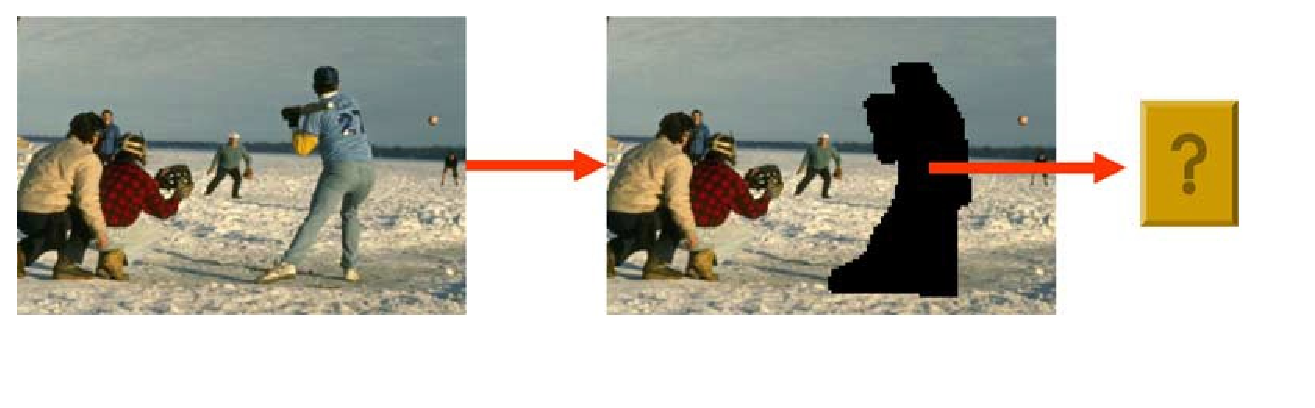
\includegraphics[width=6in]{prune1.eps}\\
  \caption{Object removal}\label{}
Object removal is just one of the many cases where image completion
needs to be applied. In the specific example shown, the user wants to remove a
person from the input image on the left. He, therefore, simply marks a region
around that person and that region must then be filled automatically so that a
visually plausible outcome is obtained.
\end{figure}
\begin{figure}
  % Requires \usepackage{graphicx}
  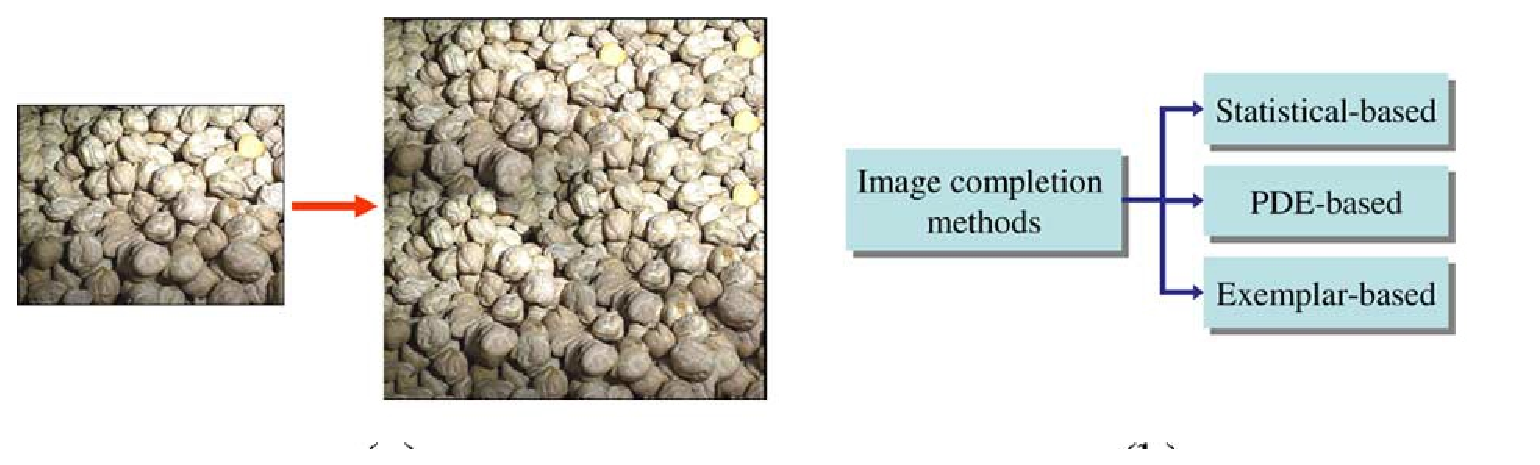
\includegraphics[width=6in]{prune2.eps}\\
  \caption{Texture synthesis problem and The three main approaches to image
Completion}\label{}
\end{figure}




\paragraph{Exemplar-Based Methods} : Exemplar-Based techniques, which actually have been the most successful techniques up to now. These methods try to fill the unknown region simply
by copying content from the observed part of the image. All exemplar-based techniques for texture synthesis
that have appeared until now, were either pixel-based or patch-based, meaning that the final texture
was synthesized one pixel, or one patch at a time (by simply copying pixels or patches from the observed image, respectively).
\\ A new exemplar-based framework  which treats image completion, texture synthesis, and image inpainting in a unified manner. All   image-editing tasks in the form of a discrete global optimization is used to avoid visually inconsistent results.
\\ The objective function of this problem is global optimization well-defined, and corresponds to the energy of a discrete Markov random field (MRF)
For efficiently optimizing this MRF, a novel optimization scheme, called priority belief propagation (BP) is used  which carries two very important extensions over the standard BP algorithm

  \begin{enumerate}
  \item \textbf{Priority-based message scheduling}
  \item \textbf{Dynamic label pruning}
\end{enumerate}

These two extensions work in cooperation to deal with the intolerable computational cost of BP, which is caused by the huge number of labels associated with  MRF. Moreover, both of  extensions are generic, since they do not rely on the use of domain-specific prior knowledge.They can, therefore, be applied to any MRF, i.e., to a very wide class of problems in image processing and computer vision.\\As one of  major limitation of the BP algorithm  is  its inefficiency in handling MRFs with very large discrete state spaces is considered to resolve by these extension techniques.

A novel optimization scheme which carries priority-based message scheduling and dynamic label pruning extensions for Belief Propagation known a priority BP is used.

The same optimization techniques can be used other types of completion problems such as video completion or geometric completion,constrained texture synthesis
\\ Priority-BP algorithm, which is a generic MRF optimization scheme can be used to other labeling problems  for which the large cardinality of their state-space causes them
to have a very high computational cost.


\section{Low Memory Cost Block-Based Belief Propagation For Stereo Correspondence}

Stereo correspondence is used in computer vision to find the depth among the cameras and objects.\\ This depth inference problem could be further transformed  to  a disparity inference problem by assuming that the cameras and objects are under epipolar geometry. The inferred disparity information could be widely applied to tracking, surveillance system, and multiview video coding \\\
The stereo matching algorithms can be roughly divided into two categories.
\\\
\begin{itemize}
  \item \textbf{local approaches}
  \item \textbf{global approaches}
\end{itemize}
\begin{itemize}
  \item Local approaches select disparities of image pixels using the information in a window. Therefore local approaches are faster than global approaches. However, it results in poor accuracy since the local approaches could not deal with textureless regions and occluded regions well due to the insufficient information in window.
  \item On the other hand, global approaches can handle the textureless and occluded regions well by formulating disparity inference as an energy minimization problem
\end{itemize}

 \begin{itemize}
   \item The energy function usually has a smoothness constraint which represents a certain physical relationship between neighboring pixel pair.
   \item This  smoothness  constraint often enforces penalty on the energy function, if the labels (disparities or segments) of neighboring pixels are inconsistent.
   \item Among the global methods, 2-D optimization algorithms such as graph cut and belief propagation (BP)  have been applied quite successfully to optimize energy function.
\end{itemize}



\begin{figure}
  % Requires \usepackage{graphicx}
  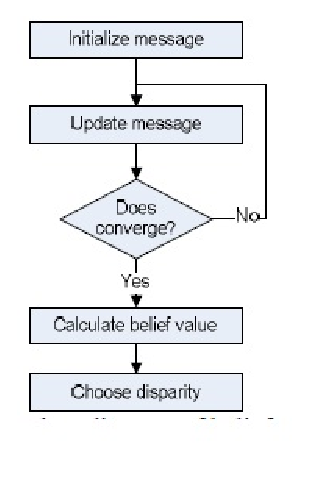
\includegraphics[width=2in]{block1.eps}\\
  \caption{Flow diagram of Belief Propagation}\label{}
\end{figure}
The flow chart  for Belief Propagation is shown in figure 3.5
 The BP algorithms construct 2-D graph structures with nodes representing all the pixels in the disparity images to find the disparity map with energy closer to the global minima.\ However, the vast number of nodes in the 2-D graph  result in  extremely high computation complexity, thereby rendering 2-D optimization is too difficult to be directly implemented for real-time application.\\
A block-based BP algorithm that directly partitions an image into separated independent blocks. Thus, can reduce the memory size significantly due to block based computation. In addition, the independent blocks also enable parallel computation by multiple computation units. Moreover earlier convergence for each block can also improve the long running time.


\begin{figure}
   Requires \usepackage{graphicx}
 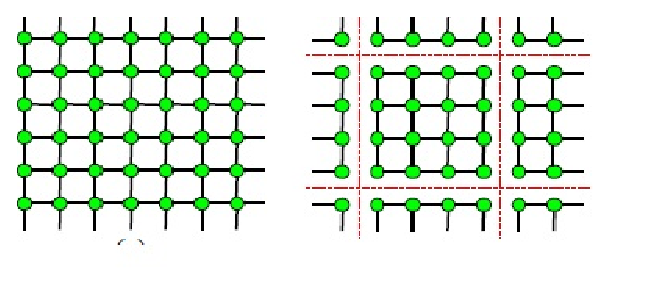
\includegraphics[width=4in]{block2.eps}\\
  \caption{graph of typical and block based BP}\label{}
2D Graph Model is shown in figure 3.6
\end{figure}

A new stereo matching algorithm partitions an image to block and optimizes with belief propagation technique.This method reduces memory storage size by 99
with good performance.
 To enhance the interaction  between neighboring blocks such that the independent block could extract useful information from  neighboring finished processing blocks are possible with block belief propagation.
\section{Task Parallel Implementation Of Belief Propagation In Factor Graphs}

Graphical models have been essential tools for probabilistic reasoning. Factor graphs  have emerged as a unified model of directed graphs (e.g. Bayesian networks) and undirected graphs (e.g. Markov networks).\\ A factor graph naturally represents a joint probability distribution that is written as a product of factors, each involving a subset of random variables.
Factor graphs have found applications in   Image processing,Bioinformatics and  Error-control decoding used in digital communications
Relation beteween  Factor graphs and Belief Propagation.
\begin{itemize}
  \item Inference is a problem of computing posterior probability distribution of certain variables given some value as observed or evidence variables.
  \item In factor graphs, inference proceeds with the well-known belief propagation algorithm . Belief propagation is a process of passing messages along the edges of a graph. Processing each message requires a set of operations with respect to the probability distribution of the random variables in a graph.
  \item Such distribution is represented by potential tables. The complexity of belief propagation increases dramatically as the number of states of variables and node degrees of a graph increase.
\end{itemize}

In many applications, such as digital communications, belief propagation must be performed in real time.\\ Therefore, parallel techniques are needed to accelerate the inference.Many parallel techniques have been proposed for belief propagation in factor graphs.\\ Parallelizing belief propagation in acyclic factor graphs still remains a challenging problem due to the precedence constraints among the nodes in the graphs. \\ Task scheduling is used in parallel computing is an efficient tool  for linear algebra problem on general-purpose multi-core processors.
The  methods used for  implementation of Belief Propagation using factor graphs are task dependency graph is used  by using a dynamic task scheduler.


\section{ Hardware-Efficient Belief Propagation}
Loopy belief  propagation (BP)  is  an  effective solution for  assigning labels to  the  nodes of  a  graphical model such as the Markov random field (MRF),
\begin{itemize}
  \item But it requires high memory, bandwidth, and computational costs.
\end{itemize}

The loopy BP has been widely applied to

\begin{itemize}
  \item Stereo matching
  \item Image denoising
  \item Image inpainting
\end{itemize}
  The success of BP is due to its regularity and simplicity. It uses a simple message  update  process  to iteratively refine the  beliefs  of labels for each node. A message sent from one node to another is updated according to neighboring messages and local energy functions, using simple arithmetic operations.\\
However, BP algorithms generally require a great amount of memory for storing the messages, typically on the order of tens to hundreds times larger than the input data.\ Besides, since each message is processed hundreds of times, the saving/loading of  messages consumes considerable bandwidth.\ Therefore, although BP may work on high-end platforms such as desktops, it cannot be applied to most consumer electronic devices that have limited memory, computational power, and energy. \ sequential procedure,  it  is  difficult to  utilize  hardware  parallelism  to accelerate BP.
The  two techniques  used
\begin{itemize}
  \item The first one is tile-based BP   splits the Markov random field (MRF) into many tiles and only stores the messages across the neighboring tiles. The memory and bandwidth required by this technique is only a fraction of the ordinary BP algorithms. But the quality of the results comparable to other efficient algorithms ,results are   tested by the publicly available Middlebury MRF benchmarks

  \item Second technique is that The fast message construction technique is based on the observation that many hypotheses used to construct the mesasages are repetitive. therefore, they only need to be computed once. This observation allows us to reduce the complexity of message construction from

\end{itemize}

Moreover, unlike previous sequential algorithms, the proposed algorithm can be easily parallelized.\
These techniques can be realized in both hardware and software. \ A software reference implementation compatible to  the  Middlebury  MRF  library  is  available  online,\ while two hardware the first one is a very large scale integration (VLSI) circuit and the second one a graphic processing unit (GPU) program are analyzed in this paper.



 The techniques used to develop a tile-based message passing and fast message construction  algorithm greatly reduced the memory, bandwidth, and computational costs of BP and enabled the parallel processing. With these two techniques  BP  can be  more suitable for low-cost and power limited consumer electronics.

\section{PMBP: PatchMatch Belief Propagation for Correspondence Field Estimation}
Patch Match is a simple, yet very powerful and successful method for optimizing Continuous labelling problems.
The algorithm has two main approaches  used are
\begin{itemize}
  \item The update of the solution space by sampling
  \item The use of the spatial neighborhood to propagate samples.
\end{itemize}
These approaches are related to steps in a specific form of belief Propagation in the continuous space, called Particle Belief Propagation (PBP). However, BP has thus far been too slow to allow complex state spaces.\\The two approaches used in this research yields a new algorithm called
Patch Match Belief Propagation for Correspondence Field estimation (PMBP), which is more accurate than Patch Match and orders of magnitude faster than PBP.
The methods used in research is novel realistic pair wise terms that provide Smoothness used for the recent Patch Match Stereo work.
The link between the popular PatchMatch method and the very well-known Belief propagation algorithm.

The link between the popular PatchMatch method and the very well-known Belief propagation algorithm  introducing additional pairwise terms, These approaches  can be  used as both in terms of applications, such as optical flow, as well as algorithms such as different forms of message passing e.g.  Treereweighted


\section{Learning continuous time Bayesian network classifiers}
Streaming data are relevant to use in finance,computer science,engineering while  they are becoming increasingly important to medicine and biology.


 The approach used for continuous time Bayesian network classifiers
  \begin{itemize}
    \item Continuous time Bayesian network classifiers are designed for analyzing multivariate streaming data when time duration of event matters.
    \item Structural and parametric learning for the class of continuous time  Bayesian network  classifiers are  considered  in  the  case where  complete  data is available.
    \item Conditional log-likelihood  scoring is developed for structural learning on continuous time Bayesian network classifiers.
   \item Results show that conditional  log-likelihood  scoring combined with Bayesian parameter estimation outperforms marginal log-likelihood scoring.
   \item Conditional log-likelihood  scoring becomes even more effective when  the amount of available data is limited.
\end{itemize}

Conditional log-likelihood scoring function is used  to learn continuous time Bayesian network classifiers from multivariate streaming  data.
Same function can be used for classifying multivariate trajectories in the case where the class is static .The quality of the classification performances also suggests to extend the Continuous Time Bayesian Network Classifiers to the clustering problem.

















\chapter{Conclusion}


The graphical representation or models for multidimentional probability distributions such as Markov  Random Fields and  Bayesian Networks are used for Belief Propagation Techniques.
Some of the applications results are obtained based on following Techniques:
Optimizing Markov  Random Fields to speed up the  Belief Propagation used for face recognition and low level vision problem

Another optimizing scheme which carries priority based message scheduling and dynamic label pruning extensions are used to handle  Markov  Random Field with large discrete space.

The block based Belief Propagation algorithm reduces memory size significantly due to block based computation.

A parallel techniques are used for implementation of Belief Propagation Techniques in acyclic  factor graphs.

A tile based Belief Propagation and fast construction techniques are realized both in Software and Hardware.

Learning continuous time Bayesian network classifiers are used for data streaming by using conditional log-likelihood scoring function.



\chapter{\textbf{Conclusion}}



The  MS PPT are used to optimize the  information under constrains and getting message across audience can be achieved by means of using less text and less special effects in each slide and the ideas and reference data are represented by data visualization methods.


%\include{chap_conclusions}      % Finally the summary & conclusions

%--------------------------------------------------------------------%
% APPENDIX
%  Appendices, if any, must precede the cited literatures.
%  Appendices shall be numbered in Roman Capitals (e.g. Appendix IV)
\appendix
%\include{appendix_1}        % Appendices if any..

%--------------------------------------------------------------------%
% LITERATURE CITED
%   This should follow the appendices, if any, otherwise summary and
%   conclusions chapter.
%\bibliography{ieeetr}              % Make the bibliography
\begin{thebibliography}{9}
\bibitem{Stephen Moffat}
Stephen Moffat
\textit{Power Point Advance 2010 }.
the mouse training company. revised edition , USA , 20013.
\bibitem{Shelley Fishel}
Shelley Fishel.
\textit{Power Point Advance 2013 }.
the mouse training company. revised edition., London.2013.

\bibitem{Negriono}
Neriono
\textit{Microsoft Office Powerpoint Visual quick Start Guide}.
Pearson Education India.New Delhi,2012
%[\textit{}].



\bibitem{Codeman Lisa }
Codeman Lisa
\textit{Microsoft Power Point }.
%[\textit{On the electrodynamics of moving bodies}].
Wikipedia, the free encyclopedia

\bibitem{Carlo satta}
 Carlo satta
 \\\texttt{http://www.presentation-process.com/powerpoint-tutorial.html/Infographics}

\bibitem {Heather Ackmann }
Heather Ackmann
\\\textit {Instructor ,Microsoft certified Master, Hyperlinks with Actions}
www.trainsignal.com. sydney

\bibitem {Varvark }
Varvark
\\\textit {Using Graphs and Tables on Presentation Slides Think Outside The Slide PowerPoint 2013 }
www.gethelp.library.upenn.edu , New York

 \bibitem{Anna willms web }
Anna willms webb
\textit{}.
\textit{Hyperlinks and Action ButtonsBrowser HTML }

\bibitem{Thomas seymat and Thomas Rickver }

Thomas seymat and Thomas Rickver
\textit{http://www.presentation-process.com/powerpoint-tutorial.html.Infographics}.
%[\textit{On the electrodynamics of moving bodies}].
\bibitem{Anna and Bob}
Anna and Bob
\textit{from goodwill community foundation,http://www.gcflearnfree.org}

\end{thebibliography}
%--------------------------------------------------------------------%
% ACKNOWLEDGMENTS
%   For APS, acknowledgements can be the first item after title page
%      OR
%   the very last item.
%
%\begin{acknowledgments}
% I thank the many people who have done lots of nice things for me.
%\end{acknowledgments}


\end{document}
